\chapter{Planning and Design}
\label{chapter5}

\section{Game Design Process}
The game design process started by using the HTC Vive to research what kind of games were already on the market for the HTC Vive. The games that were SteamVR Demo\cite{steamvr}, The Lab\cite{thelab}, Space Pirate Trainer\cite{spacepiratetrainer}, and Elite Dangerous\cite{elitedangerous}. This research was done in order to give a feel for the HTC Vive and it's capabilities, this would give a clearer understanding to which kind of games are more suited to the Virtual Reality platform.
\newline
\par
The next step in the game design process was to brainstorm ideas of what kind of game would be made for the project. The ideas would be split into four categories, these four categories are the theme of the game, the features of the game, the genre of the game, and the benefits of the game as seen in the whitebaord Figure \ref{fig:brainstorm} and the table bersion in Figure \ref{fig:brainstormtable}.

\begin{figure}[H]
	\includegraphics[width=\textwidth]{brainstorm}
	\centering
	\caption{Image showing the whiteboard brainstorm for demo ideas.}
	\label{fig:brainstorm}
\end{figure}

\begin{figure}[ht]
	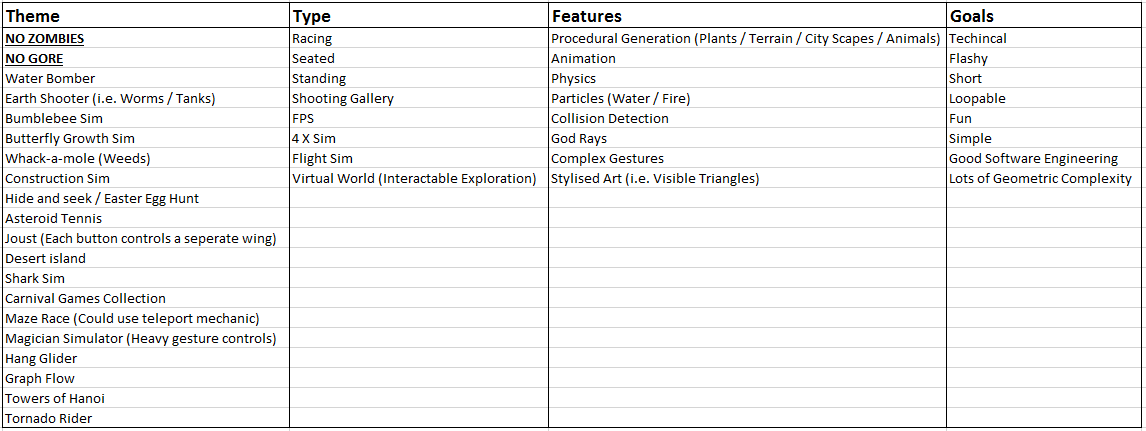
\includegraphics[width=\textwidth]{brainstormtable}
	\centering
	\caption{Table showing the brainstorm for demo ideas.}
	\label{fig:brainstormtable}
\end{figure}

\clearpage
The brainstorm was then categorised in a separate table, combining the ideas that have relevance together, this table can be seen in \ref{fig:narrowedtable}.

\begin{figure}[H]
	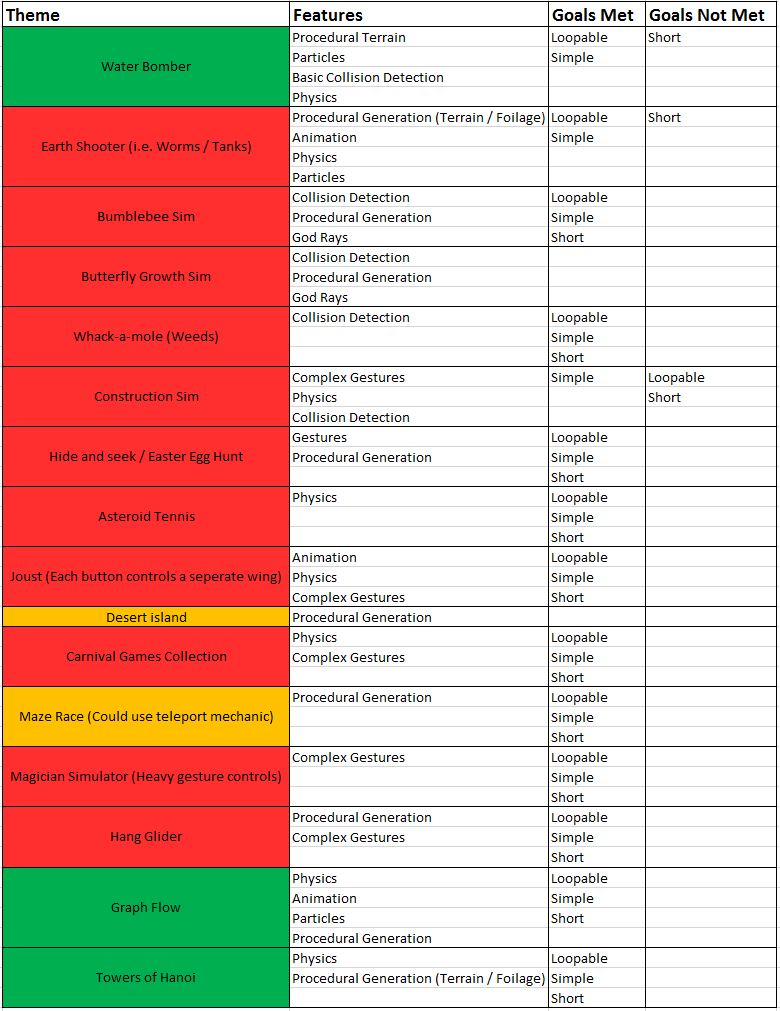
\includegraphics[width=12cm]{narrowedtable}
	\centering
	\caption{Table showing brainstorm ideas categorised and coloured depending on how probable it would be used.}
	\label{fig:narrowedtable}
\end{figure}

Then using the updated table of ideas, the ideas were narrowed down until one that could feasibly done was chosen out of all the ideas on the white-board. This idea was to combine the Towers of Hanoi and Graph Flow in a puzzle game. These two ideas were combined in order to make a technology demonstration that is very specific to the School of Computing in the University of Leeds, as these are both topics of study during the Computer Science course in the university of Leeds.
\newline
\par
A goal for the game then had to be designed. The goal of the game was decided to be having the right amount of flow run down to set nodes, where flowers would be. If these flowers have too much water flow they would look dead, and if they had too little water flow they would also look dead. They would only look alive if the water flow was the correct amount. The game is won when all the flowers are "alive" at the same time.
\newline
\par
This idea would implement many non-trivial features in the Unreal Engine, such as:
\begin{itemize}
	\item Randomly generating a graph
	\item Generating a terrain based on the graph
	\item Towers of Hanoi logic for flow control
	\item Having plants being affected by the water flow
	\item Changing the appearance of the water, based on the flow of that edge of the graph
\end{itemize}


\section{Virtual Reality Features}
The Virtual reality Features that will be used are:
\begin{itemize}
	\item Using the Head Mounted Display in order to look around the virtual world.
	\item Using the controllers to pick up the Towers of Hanoi disks, and place them down.
	\item Using the controllers to select a teleport location to move.
\end{itemize}

\section{Graph Flow}
Graph Flow will be used in this technical demonstration as the main objective of the game. The objective of the game will be to get the flow to match the goal flow. This will be done by blocking off certain rivers to redirect flow from one river into another. The goal flow will be calculated in development, and each level that is created will also have a goal state completed.

\section{Towers of Hanoi}
Towers of Hanoi will be used in the demo to block off the graph flow from nodes to other nodes. This will be done by having rods in the river at each split in the graph. These will be placed at the output of each split in the river. The Towers of Hanoi disks will then be placed on top of these rods if the flow needs to be blocked. The Towers of Hanoi disks will only be allowed to be placed in the opposite order compared to the way the normally are. This would mean that a larger disk can only be placed on top of a smaller disk. This order had to be inverted to the standard as rivers are narrower at the bottom, compared to the top of the river ditch. 

\section{Plant Survival}
The Plant Survival will be used as a measure for the player to determine how close he is to solving the puzzle. This will be the indicator to the player if the flow at that node matches the pre-determined flow for the level